% Estimation Flowcharts: NFXP vs RL-Based Structural Estimation
% Chapter 5: Solving Economic Models with RL
% Standalone TikZ diagram — compile with: pdflatex estimation_flowcharts.tex

\documentclass[tikz,border=8pt]{standalone}
\usepackage{amsmath,amssymb}
\usetikzlibrary{arrows.meta, positioning, calc, fit, backgrounds, decorations.pathreplacing}

% Project palette (from docs/compile_chapter.tex)
\definecolor{rlblue}{HTML}{4878A8}
\definecolor{rlorange}{HTML}{D4915C}
\definecolor{rlgreen}{HTML}{6BA368}
\definecolor{rlred}{HTML}{C25B56}
\definecolor{rlpurple}{HTML}{8B7BAF}
\definecolor{rlgray}{HTML}{888888}
\definecolor{rlblack}{HTML}{2D2D2D}

\begin{document}
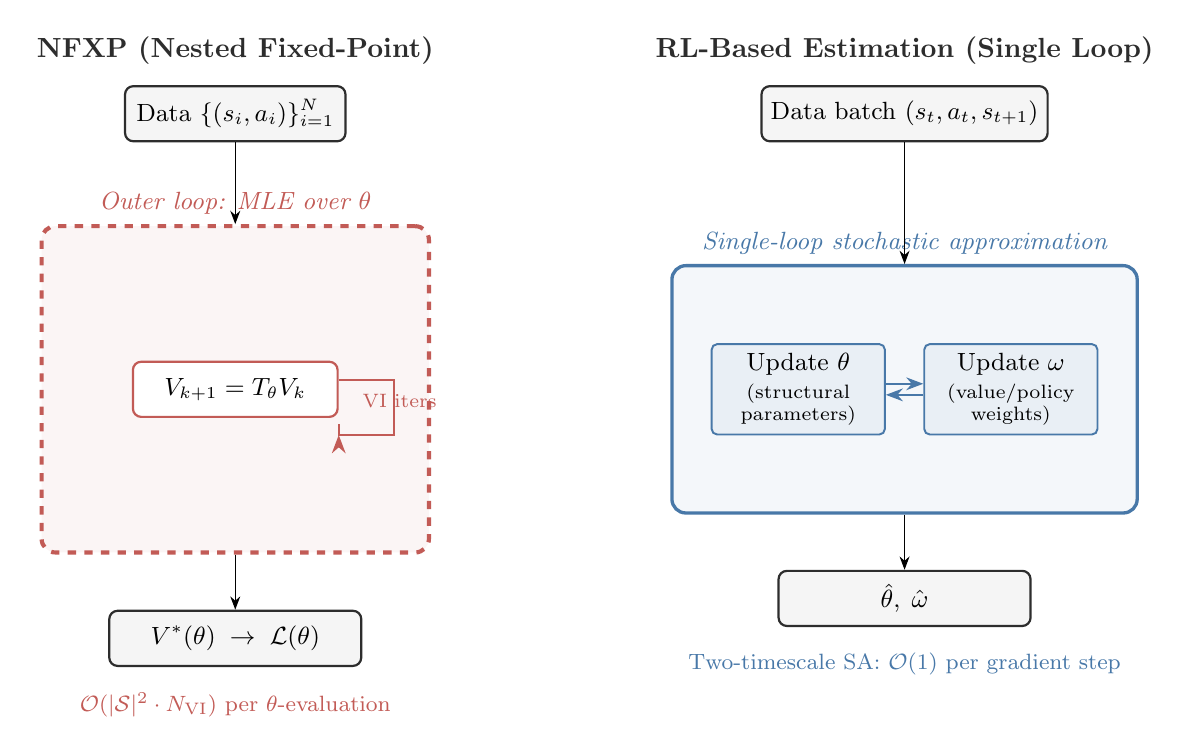
\begin{tikzpicture}[
    >=Stealth,
    node distance=0.9cm and 1.2cm,
    box/.style={
        draw=rlblack, rounded corners=3pt, minimum width=2.8cm,
        minimum height=0.7cm, align=center, font=\small,
        fill=white, line width=0.8pt
    },
    databox/.style={
        box, fill=black!4
    },
    outputbox/.style={
        box, fill=black!4, minimum width=3.2cm
    },
    innerbox/.style={
        draw=none, rounded corners=2pt, minimum width=2.0cm,
        minimum height=0.85cm, align=center, font=\small,
        fill=rlblue!12, line width=0.7pt
    },
    container/.style={
        draw=#1, rounded corners=5pt, line width=1.2pt,
        fill=#1!6, inner sep=10pt
    },
    container/.default={rlblack},
    selfarrow/.style={
        ->, >=Stealth, line width=0.8pt, color=#1
    },
    selfarrow/.default={rlred},
    every edge/.style={draw, ->, >=Stealth, line width=0.8pt},
    annotation/.style={font=\footnotesize, text=rlgray},
    panel title/.style={font=\bfseries\normalsize, text=rlblack},
]

% ===================================================================
% LEFT PANEL — NFXP
% ===================================================================
\begin{scope}[local bounding box=left panel]

    % Panel title
    \node[panel title] (title-l) at (0, 5.6) {NFXP (Nested Fixed-Point)};

    % Data input
    \node[databox] (data-l) at (0, 4.8)
        {Data $\{(s_i, a_i)\}_{i=1}^N$};

    % Bellman update box (innermost)
    \node[box, draw=rlred, minimum width=2.6cm] (bellman) at (0, 1.3)
        {$V_{k+1} = T_\theta V_k$};

    % Inner container: Bellman solve
    \begin{scope}[on background layer]
        \node[container=rlred, fit=(bellman),
              inner xsep=14pt, inner ysep=20pt,
              label={[font=\small\itshape, text=rlred]above:Inner loop: Bellman equation}
        ] (inner) {};
    \end{scope}

    % Self-loop on Bellman box (VI iterations)
    \draw[selfarrow=rlred]
        (bellman.east) ++(0, 0.12) coordinate (loop-start)
        -- ++(0.7, 0)
        -- ++(0, -0.7)
        -- ++(-0.7, 0)
        coordinate (loop-end)
        -> (bellman.east |- loop-end);
    \node[font=\scriptsize, text=rlred, right=0.18cm of bellman.east, yshift=-0.15cm]
        {VI iters};

    % Outer container: MLE loop
    \begin{scope}[on background layer]
        \node[container=rlred, dashed, line width=1.5pt,
              fit=(inner)(bellman),
              inner xsep=18pt, inner ysep=28pt,
              label={[font=\small\itshape, text=rlred]above:Outer loop: MLE over $\theta$}
        ] (outer) {};
    \end{scope}

    % Output
    \node[outputbox, below=0.7cm of outer] (output-l)
        {$V^*(\theta) \;\to\; \mathcal{L}(\theta)$};

    % Edges
    \draw[->] (data-l) -- (outer.north);
    \draw[->] (outer.south) -- (output-l);

    % Complexity annotation
    \node[annotation, text=rlred, below=0.2cm of output-l]
        {$\mathcal{O}(|\mathcal{S}|^2 \cdot N_{\mathrm{VI}})$ per $\theta$-evaluation};

\end{scope}

% ===================================================================
% RIGHT PANEL — RL-Based Estimation
% ===================================================================
\begin{scope}[xshift=8.5cm, local bounding box=right panel]

    % Panel title
    \node[panel title] (title-r) at (0, 5.6) {RL-Based Estimation (Single Loop)};

    % Data input
    \node[databox, minimum width=3.2cm] (data-r) at (0, 4.8)
        {Data batch $(s_t, a_t, s_{t+1})$};

    % Inner boxes: theta and omega updates
    \node[innerbox, draw=rlblue, line width=0.7pt, minimum width=2.2cm, minimum height=1.1cm]
        (theta) at (-1.35, 1.3)
        {Update $\theta$\\[-1pt]{\scriptsize(structural}\\[-3pt]{\scriptsize parameters)}};

    \node[innerbox, draw=rlblue, line width=0.7pt, minimum width=2.2cm, minimum height=1.1cm]
        (omega) at (1.35, 1.3)
        {Update $\omega$\\[-1pt]{\scriptsize(value/policy}\\[-3pt]{\scriptsize weights)}};

    % Bidirectional coupling arrows
    \draw[->, rlblue, line width=0.7pt]
        ([yshift=2pt]theta.east) -- ([yshift=2pt]omega.west);
    \draw[->, rlblue, line width=0.7pt]
        ([yshift=-2pt]omega.west) -- ([yshift=-2pt]theta.east);

    % Main container: single-loop SA
    \begin{scope}[on background layer]
        \node[container=rlblue,
              fit=(theta)(omega),
              inner xsep=14pt, inner ysep=28pt,
              label={[font=\small\itshape, text=rlblue]above:Single-loop stochastic approximation}
        ] (main) {};
    \end{scope}

    % Output
    \node[outputbox, below=0.7cm of main] (output-r)
        {$\hat{\theta},\; \hat{\omega}$};

    % Edges
    \draw[->] (data-r) -- (main.north);
    \draw[->] (main.south) -- (output-r);

    % Complexity annotation
    \node[annotation, text=rlblue, below=0.2cm of output-r]
        {Two-timescale SA: $\mathcal{O}(1)$ per gradient step};

\end{scope}

\end{tikzpicture}
\end{document}
